\documentclass[a4paper,12pt]{article}

% Pacotes úteis
\usepackage[utf8]{inputenc}       % Codificação UTF-8
\usepackage[T1]{fontenc}          % Suporte para acentuação
\usepackage{lmodern}              % Fonte moderna
\usepackage{graphicx}             % Para inclusão de imagens
\usepackage{amsmath}              % Pacote de matemática
\usepackage{amssymb}              % Símbolos matemáticos
\usepackage{geometry}             % Controle das margens
\usepackage{setspace}             % Controle de espaçamento
\usepackage{indentfirst}          % Indentar primeiro parágrafo de cada seção
\usepackage{hyperref}             % Links clicáveis
\usepackage{float}                % Controle de posição de elementos flutuantes (figuras, tabelas)
\usepackage{titlesec}             % Personalização de títulos
         % Para imagens (caso use)
\usepackage{xcolor}           % Para cores nos textos (opcional)
\usepackage{listings}         % Para código C++ (se for incluir trechos)



\documentclass{article}
\usepackage{minted}

% Configurações opcionais para personalizar
\setminted{
    breaklines=true,      % Quebra automaticamente linhas longas
    breakanywhere=true,   % Permite quebrar palavras (opcional)
    frame=lines,          % Adiciona linhas ao redor do código
    fontsize=\small,      % Tamanho da fonte
    breaklines=true,
    breaksymbol=,         % Adiciona um símbolo (opcional)
    breakindent=10pt       % Indenta as linhas quebradas
}



% Configurações de página
% \geometry{left=3cm, right=2cm, top=2cm, bottom=2cm}
% \onehalfspacing                      % Espaçamento de 1,5 entre linhas

% % Cabeçalho com título e autores
% \title{Avaliação de LLM's na extração de dados médicos de notas clínicas}
% \author{
%     Ana Júlia Amaro Pereira Rocha \\ 
%     Maria Eduarda Mesquita Magalhães\\ 
%     Mariana Fernandes Rocha \\ 
%     Paula Eduarda de Lima \\
%     \\ Orientador: Walter Sande
% }
% \date{\today}                         % Data do relatório

% \begin{document}

% \documentclass[12pt,a4paper]{report}
\usepackage{graphicx}
\usepackage{titling}

\documentclass[a4paper,12pt]{article}

\usepackage[portuguese]{babel} % Ativa o português para hifenização
\usepackage[utf8]{inputenc}    % Suporte a caracteres acentuados
\usepackage[T1]{fontenc}       % Fonte com suporte a caracteres especiais

\begin{document}

\begin{titlepage}
    \begin{center}

        \vspace{1cm}
        \begin{minipage}{0.45\textwidth}
            \centering
            
\includegraphics[width=1.2\textwidth]{logo_fgv.png}    
        \end{minipage}
        \vspace{2cm}

        \rule{1\textwidth}{0.4pt} \\ % Linha horizontal personalizada
        \vspace{0.3cm}
        {\Huge \textbf{Projeto de Micro-Framework}} \\
        \vspace{0.2cm}
        \vspace{0.5cm}\\
        {\Large \textbf{A1 Computação Escalável}}\\
        \rule{1\textwidth}{0.4pt} % Linha horizontal personalizada


        \vspace{0.5cm}
        {\Large \textbf{FGV EMAp}} \\
        \vspace{2cm}
        
        

        
        
        % % Unidade e curso
        % {\Large \textbf{FGV EMAp}}\\[2cm]
        
        % Autores
        {\large 
            \textbf{Ana Júlia Amaro Pereira Rocha} \\ 
            \textbf{Maria Eduarda Mesquita Magalhães}\\
            \textbf{Mariana Fernandes Rocha} \\
            \textbf{Paula Eduarda de Lima}}\\[1.5cm]
        
        % Informações adicionais
        {\large 
            Ciência de Dados e Inteligência Artificial \\ 
            5º Período}\\[2cm]
        
         % Data
        \vfill
        {\large Rio de Janeiro, 2025}

        
    \end{center}
\end{titlepage}

\tableofcontents
\newpage


\section{Introdução}
Este relatório apresenta o desenvolvimento de um Micro-Framework voltado à construção de pipelines para processamento de dados. O principal objetivo é fornecer uma solução que promova maior eficiência e balanceamento de carga, por meio da execução concorrente e paralela das etapas de processamento. Embora a aplicação tenha sido especialmente construida para o monitoramento de uma doença infecciosa, sua estrutura foi projetada de forma genérica, com pontos de extensão (hot-spots) que permitem a personalização conforme as necessidades específicas de diferentes cenários.

\section{Modelagem}

\begin{figure}[H]
    \hspace{-1cm}
    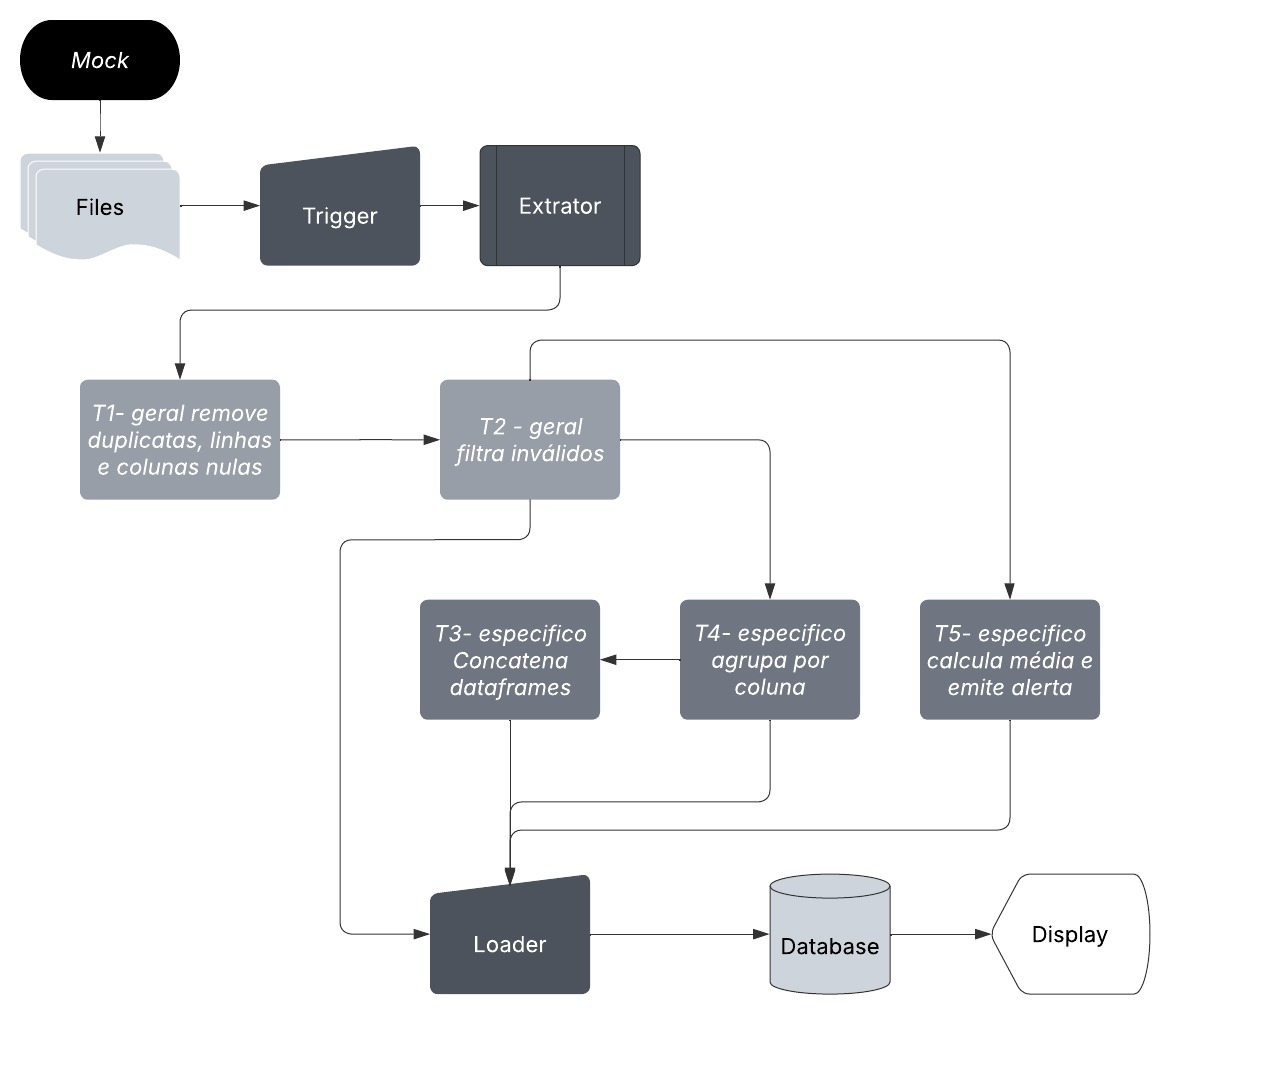
\includegraphics[width=1.15\linewidth]{Fluxograma.jpeg}
    \caption{Fluxograma do framework}
    \label{fig:minha_imagem}
\end{figure}

A modelagem, representada no fluxograma, é feita de um pipeline de processamento de dados baseado em um fluxo ETL (Extract, Transform, Load), acionado por diferentes triggers, organizado em etapas independentes, que se comunicam por meio de filas. O processo se inicia por um módulo mock que simula a chegada de dados reais de fontes distintas. Esses dados são armazenados em arquivos e enviados para a primeira etapa do pipeline.

Quando o pipeline é ativado por um dos triggers, os arquivos são encaminhados para o extrator, que é responsável por identificar o tipo de arquivo e padronizar os dados extraídos em uma estrutura de dataframe. Esse processo garante que, independentemente do formato de origem, todos os dados estejam organizados de maneira uniforme para as próximas etapas do pipeline.

Após a extração, os dados passam por uma cadeia de tratadores gerais, que realizam limpezas e filtragens padronizadas, T1, T2, e T3 - geral.

Na sequência, os dados seguem para tratadores específicos, que aplicam transformações mais contextualizadas. O T1 - específico concatena diferentes DataFrames, unificando tabelas com a mesma estrutura. O T2 - específico realiza agrupamentos por colunas de interesse (como CEP ou hospital), preparando os dados para análises agregadas. Por fim, o T3 - específico calcula médias e outras estatísticas relevantes, oferecendo uma visão resumida dos dados processados.

Após o tratamento, os dados são encaminhados para o Loader, responsável por carregá-los em arquivos csv's. Isso garante que os dados tratados fiquem disponíveis para consultas futuras e possam ser utilizados por módulos de visualização. Por fim, o componente Display consome essas informações armazenadas e as exibe relatórios semanais, fechando o ciclo do pipeline. 

\section{Mock}

As fontes de dados serão simulações de hospitais,  Secretaria de Saúde (SS) e Organização Mundial da Saúde (OMS). Receberemos conjuntos de dados advindos dessas fontes semanalmente. Além disso, temos dois tipos de segmentação regional: Ilhas, mais geral, e regiões, que são segmentações das ilhas, mais especifíco. A simulação apresenta 20 ilhas, cada uma identificada por um CEP de 2 dígitos, cada ilha tem 5 regiões, com CEPs de 5 dígitos, sendo os dois primeiros dígitos o CEP da ilha (ex: ilha 12 $\rightarrow$ regiões 12001 a 12005).


O objeto Mock é feito em python e implementa a criação de três tipos de tabelas diferes: SQLite, csv e txt.
\vspace{0.5cm}

\textbf{Fontes e dados gerados}

\begin{itemize}
    \item \textcolor{purple}{\textbf{OMS (\texttt{oms\_mock.txt})}}\\
    Dados agregados por ilha (CEP de 2 dígitos).\\
    Inclui número de óbitos, população, recuperados, vacinados e data.\\
    Gerado em formato \texttt{.txt} com tabulações.
    
    \vspace{0.5em}
    
    \item \textcolor{red}{\textbf{Hospitais (\texttt{hospital\_mock\_*.csv})}}\\
    Dados individuais por paciente, com CEPs de 5 dígitos (regiões).\\
    Contém informações como internação, idade, sexo, sintomas e data.\\
    Gera múltiplos arquivos \texttt{.csv}, simulando diferentes hospitais.
    
    \vspace{0.5em}
    
    \item \textcolor{orange}{\textbf{Secretaria de Saúde (\texttt{secretary\_data.db})}}\\
    Banco de dados SQLite com tabela \texttt{pacientes}.\\
    Dados por região (CEP de 5 dígitos): diagnóstico, vacinação, escolaridade, população e data.\\
    Registros inseridos diretamente em um banco relacional.
\end{itemize}

\section{Triggers}
O framework apresenta dois tipos de Triggers responsáveis por iniciar a execução de um pipeline:

\begin{itemize}
    \item \textbf{TimerTrigger}: A cada X segundos dispara uma nova execução.
    \item \textbf{RequestTrigger}: A cada chamada de função (simulando uma requisição de rede) dispara uma nova
execução.
\end{itemize}

\section{Extrator}

O  extrator, implementado em C++, usa a classe \texttt{DataFrame} que organiza os dados gerados pelo mock em uma estrutura tabular com colunas bem definidas e suporta os diferentes tipos de dados (inteiros, reais e strings). Ele permite:

\begin{itemize}
    \item \textbf{Validar os dados inseridos:} garante que cada valor esteja no formato correto (ex: inteiros em colunas inteiras).
    
    \item \textbf{Adicionar ou remover linhas e colunas:} facilita manipulações e filtragens nos dados carregados.
    
    \item \textbf{Visualizar os dados em forma de tabela:} com o método \texttt{display}, os dados são impressos com cabeçalho e valores formatados.
    
    \item \textbf{Acessar partes específicas:} como uma linha (\texttt{getRow}) ou coluna (\texttt{colIdx} e \texttt{typeCol}).
    
    \item \textbf{Verificar informações básicas:} número de colunas (\texttt{numCols}), número de linhas (\texttt{size}), se está vazio (\texttt{empty}), etc.
\end{itemize}

\vspace{1em}

\textbf{Aplicação com os dados gerados}
\\
\\
O extrator identifica o tipo de arquivo da tabela em questão por meio da extensão pós ponto (.csv,.txt ou .db) e, com isso, chama a respectiva função de extração para esse tipo de dado, tornando os diferentes tipos de tabelas padronizadas para o uso dos tratadores.\\
\\
Quando os dados da OMS (arquivo \texttt{.txt}) ou dos hospitais (arquivos \texttt{.csv}) são carregados, o \texttt{DataFrame} pode ser inicializado com os nomes das colunas e seus tipos, e cada linha é validada antes de ser inserida.
\\
\\
O extrator também pode ser usado para representar tabelas extraídas do banco de dados SQLite da Secretaria de Saúde (por exemplo, a tabela \texttt{pacientes}).
\\
\\
Ele garante integridade dos dados e fornece uma base comum para as análises posteriores.


\section{Tratadores}
\subsection{T1}
\subsection{T2}
\subsection{T3}
\subsection{T4}
\subsection{T5}
\subsection{T6}


\section{Loader}


\section{Dashboard}

\section{Pipeline}
O Pipeline é feito de modo a organizar o fluxo de trabalho de maneira eficiente e paralela. O objetivo principal é o passo a passo dejado do ETL e a escolha da ordem e dos diferentes tratadores desejados. Além disso,essa arquitetura pode ser adaptada para qualquer outro contexto de processamento de dados.

\subsection*{Lógica Produtor-Consumidor}
De maneira geral, o paralelismo no pipeline se dá pela lógica de Produtor-Consumidor, da seguinte forma:
\\
\\
\textbf{Produtor}: gera dados e os insere em uma fila compartilhada.
\\
\\
\textbf{Consumidor}: retira dados dessa fila para processá-los.
\\
\\
\textbf{Fila compartilhada}: estrutura de dados para comunicação entre threads.
\\
\\
\textbf{Mutex (trava)}: garante que só uma thread acesse a fila por vez.
\\
\\
\textbf{Condition Variable}: notifica consumidores quando há dados disponíveis (ou produtores quando há espaço, se necessário).



\subsection*{Extração}
O paralelismo na extração dos arquivos gerados pelo mock no pipeline é implementado com base no modelo produtor-consumidor utilizando threads, filas protegidas por mutex, e variáveis de condição para sincronização.

\begin{itemize}
    \item Produtor coloca arquivos na fila (filaArquivos).

    \item  Múltiplos consumidores-extratores (threads) consomem essa fila paralelamente (o número de consumidores é um argumento da função pipeline, definido como preferível).

    \item  Cada consumidor-extrator:
    \begin{itemize}
        \item Lê o arquivo (pode ser .csv, .txt, ou .db).
        \item Constrói um DataFrame.
        \item Envia esse DataFrame para a próxima etapa (extratorTratadorFila), que será tratada por outra thread.
    \end{itemize}

\end{itemize}

Múltiplas threads \texttt{consumidorExtrator} são criadas (na função \texttt{executarPipeline}).

Cada thread opera de forma independente, competindo por arquivos na fila \texttt{filaArquivos}, gerando uma condição de corrida, corrigida por uma proteção da fila com mutex.
 
Isso permite que vários arquivos sejam processados \textbf{simultaneamente} por diferentes núcleos da CPU e haja um balanceamento de carga.
\\
\subsubsection*{Pontos fortes da abordagem}
\\
\begin{itemize}
    \item \textbf{Escalabilidade com threads:} permite processar múltiplos arquivos simultaneamente, aproveitando melhor os múltiplos núcleos da CPU, o que acelera a etapa de extração.

    \item \textbf{Balanceamento automático de carga:} como os consumidores competem por arquivos na fila, a distribuição é feita de forma natural e eficiente, sem divisão manual de tarefas.

    \item \textbf{Desacoplamento entre etapas:} o uso de filas entre as fases (extração, tratamento e carregamento) permite que cada parte do pipeline opere de forma independente, evitando gargalos.

    \item \textbf{Modelo confiável:} o padrão produtor-consumidor com mutex e variáveis de condição é amplamente utilizado e considerado seguro para aplicações concorrentes.

    \item \textbf{Paralelismo configurável:} o número de consumidores pode ser definido por parâmetro na execução, facilitando testes e adaptações ao ambiente de hardware.

    \item \textbf{Sincronização segura:} uso correto de \texttt{mutex} e \texttt{condition\_variable} impede condições de corrida no acesso às filas compartilhadas.
\end{itemize}

\vspace{1em}

\\
\subsubsection*{Pontos fracos da abordagem}

\begin{itemize}
    \item \textbf{Overhead de gerenciamento de threads:} quando há muitos arquivos pequenos, o custo de criação e sincronização de threads pode superar os ganhos do paralelismo.

    \item \textbf{Ausência de priorização de arquivos:} a fila segue uma lógica FIFO simples, não considerando arquivos urgentes ou mais pesados que poderiam ser tratados primeiro.

    \item \textbf{Fila sem limite de tamanho:} caso a leitura seja muito mais rápida que o tratamento, a fila intermediária pode crescer indefinidamente e consumir muita memória.

    \item \textbf{Threads ociosas em cenários com poucos arquivos:} se a carga for baixa, as threads de extração encerram rapidamente e não são reaproveitadas.

    \item \textbf{Bloqueio com variáveis de condição:} consumidores ficam bloqueados esperando arquivos, o que pode causar ineficiência em cenários com picos esparsos de chegada de dados.

\end{itemize}

\subsection*{Tratamento}
\\



\subsubsection*{Pontos fracos da abordagem}
\\
\begin{itemize}
    \item \textbf{} 
    
\end{itemize}

\vspace{1em}

\\
\subsubsection*{Pontos fracos da abordagem}

\begin{itemize}
    \item \textbf{} 

\end{itemize}


\subsection*{Loader}
\\



\subsubsection*{Pontos fracos da abordagem}
\\
\begin{itemize}
    \item \textbf{} 
    
\end{itemize}

\vspace{1em}

\\
\subsubsection*{Pontos fracos da abordagem}

\begin{itemize}
    \item \textbf{} 

\end{itemize}



\subsection*{Dashboard}

\section{Análise de tempo de execução}
\end{document}
